\chapter{Opis projektnog zadatka}
		
		%\textbf{\textit{dio 1. revizije}}\\
		
		%\textit{Na osnovi projektnog zadatka detaljno opisati korisničke zahtjeve. Što jasnije opisati cilj projektnog zadatka, razraditi problematiku zadatka, dodati nove aspekte problema i potencijalnih rješenja. Očekuje se minimalno 3, a poželjno 4-5 stranica opisa.	Teme koje treba dodatno razraditi u ovom poglavlju su:}
		%\begin{packed_item}
			%\item \textit{potencijalna korist ovog projekta}
			%\item \textit{postojeća slična rješenja (istražiti i ukratko opisati razlike u odnosu na zadani zadatak). Dodajte slike koja predočavaju slična rješenja.}
			%\item \textit{skup korisnika koji bi mogao biti zainteresiran za ostvareno rješenje.}
			%\item \textit{mogućnost prilagodbe rješenja }
			%\item \textit{opseg projektnog zadatka}
			%\item \textit{moguće nadogradnje projektnog zadatka}
		%\end{packed_item}
		
		%\textit{Za pomoć pogledati reference navedene u poglavlju „Popis literature“, a po potrebi konzultirati sadržaj na internetu koji nudi dobre smjernice u tom pogledu.}

		Cilj je projektnog zadatka razviti web-aplikaciju koja bi sudionicima stručne konferencije poboljšala ukupan doživljaj konferencije te im raznim funkcionalnostima olakšala prisustvovanje. Funkcionalnosti koje bi omogućile izvrsno korisničko iskustvo su mogućnost direktnog video praćenja konferencije u glavnoj konferencijskoj dvorani, dio s informacijama o mjestu održavanja konferencije koji između ostalog sadrži podatke o trenutnim vremenskim uvjetima i vremenskoj prognozi za navedenu lokaciju, pregled fotografija s konferencije i lokalno pohranjivanje na vlastiti uređaj te pregled i korištenje promotivnih materijala pokrovitelja. Među istaknutim je funkcionalnostima pregled radova - postera ili prezentacija - ostalih sudionika i mogućnost ocjenjivanja onog rada za kojeg smatraju da je najbolji. Budući da organizatori stručnih konferencija ciljaju na što veći broj sudionika, razvojem aplikacije svakako bi postigli veći doseg jer bi se konferenciji moglo priključiti s bilo koje lokacije i u bilo kojem vremenu unutar ukupnog trajanja konferencije.\\

        Sistemski administrator zadužen je za proces prijave odnosno on prijavljuje autore i njihove radove nakon što mu autori koji sudjeluju na stručnoj konferenciji elektroničkom poštom pošalju sve potrebne materijale. Sistemski administrator može definirati sve potrebne uvjete za ispravan rad sustava.\\

        Prilikom dolaska na stručnu konferenciju sudionici prijavljuju svoj dolazak te pritom dobivaju lozinku za pristup toj određenoj stručnoj konferenciji na web-aplikaciji. Ukoliko sudionik odluči koristiti web-aplikaciju pri njenom otvaranju unosi lozinku koju je dobio jer je ona jedinstveni identifikator konferencije koju je posjetio. Nakon unosa lozinke otvara mu se mogućnost samostalne registracije u sustav kako bi mogao pristupiti svim funkcionalnostima i pogodnostima aplikacije.\\\\

        \textbf{Za samostalnu registraciju u sustav potrebno je sljedeće:}
        \begin{itemize}
            \item \textit{Adresa elektroničke pošte}
            \item \textit{Lozinka}
        \end{itemize}

        \textbf{Nakon registracije u sustav korisniku je dostupno sljedeće:}
        \begin{itemize}
            \item \textit{Direktno video praćenje trenutnih događanja u glavnoj konferencijskoj dvorani}
            \item \textit{Prikaz svih prijavljenih radova}
            \item \textit{Glasanje za najbolji rad po vlastitom izboru unutar vremenskog okvira}
            \item \textit{Izabrane fotografije s konferencije koje je moguće preuzeti na vlastiti uređaj}
            \item \textit{Promotivni materijali pokrovitelja konferencije}
            \item \textit{Prikaz informacija o mjestu održavanja konferencije i podatci o trenutnim vremenskim uvjetima i vremenskoj prognozi za navedenu lokaciju}
            \item \textit{Rezultati glasovanja za najbolji poster (\underbar{nakon završetka glasovanja})}
        \end{itemize}

		Sudionici stručne konferencije tijekom određenog vremenskog razdoblja koje je određeno danima i vremenom održavanja konferencije mogu glasovati za rad koji predstavlja pojedinog predavača na konferenciji. Svi radovi prikazani su u web-aplikaciji. Svaki sudionik može glasovati samo jednom odnosno za samo jedan rad za kojeg smatra da je najbolji. Ukoliko se sudionik predomisli te želi dati glas drugom radu to može učiniti ukoliko to odluči dok glasovanje još traje. Po završetku glasovanja objavljuju se rezultati koji su dostupni svim registriranim korisnicima i šalje se obavijest autorima o rangu njihovog rada prema glasovima sudionika. Porukom elektroničke pošte na dodjelu nagrade poziva se autore prva tri rada s najviše glasova, a sve se ostale sudionike također elektroničkom poštom obavještava o mjestu i vremenu dodjele nagrade. Nakon završetka glasovanja rezultati se objavljuju na web-aplikaciji u obliku rang tablice.
		
		\eject
		
		\section{Primjeri u \LaTeX u}
		
		\textit{Ovo potpoglavlje izbrisati.}\\

		U nastavku se nalaze različiti primjeri kako koristiti osnovne funkcionalnosti \LaTeX a koje su potrebne za izradu dokumentacije. Za dodatnu pomoć obratiti se asistentu na projektu ili potražiti upute na sljedećim web sjedištima:
		\begin{itemize}
			\item Upute za izradu diplomskog rada u \LaTeX u - \url{https://www.fer.unizg.hr/_download/repository/LaTeX-upute.pdf}
			\item \LaTeX\ projekt - \url{https://www.latex-project.org/help/}
			\item StackExchange za Tex - \url{https://tex.stackexchange.com/}\\
		
		\end{itemize} 	


		
		\noindent \underbar{podcrtani tekst}, \textbf{podebljani tekst}, 	\textit{nagnuti tekst}\\
		\noindent \normalsize primjer \large primjer \Large primjer \LARGE {primjer} \huge {primjer} \Huge primjer \normalsize
				
		\begin{packed_item}
			
			\item  primjer
			\item  primjer
			\item  primjer
			\item[] \begin{packed_enum}
				\item primjer
				\item[] \begin{packed_enum}
					\item[1.a] primjer
					\item[b] primjer
				\end{packed_enum}
				\item primjer
			\end{packed_enum}
			
		\end{packed_item}
		
		\noindent primjer url-a: \url{https://www.fer.unizg.hr/predmet/proinz/projekt}
		
		\noindent posebni znakovi: \# \$ \% \& \{ \} \_ 
		$|$ $<$ $>$ 
		\^{} 
		\~{} 
		$\backslash$ 
		
		
		\begin{longtblr}[
			label=none,
			entry=none
			]{
				width = \textwidth,
				colspec={|X[8,l]|X[8, l]|X[16, l]|}, 
				rowhead = 1,
			} %definicija širine tablice, širine stupaca, poravnanje i broja redaka naslova tablice
			\hline \SetCell[c=3]{c}{\textbf{naslov unutar tablice}}	 \\ \hline[3pt]
			\SetCell{LightGreen}IDKorisnik & INT	&  	Lorem ipsum dolor sit amet, consectetur adipiscing elit, sed do eiusmod  	\\ \hline
			korisnickoIme	& VARCHAR &   	\\ \hline 
			email & VARCHAR &   \\ \hline 
			ime & VARCHAR	&  		\\ \hline 
			\SetCell{LightBlue} primjer	& VARCHAR &   	\\ \hline 
		\end{longtblr}
		

		\begin{longtblr}[
				caption = {Naslov s referencom izvan tablice},
				entry = {Short Caption},
			]{
				width = \textwidth, 
				colspec = {|X[8,l]|X[8,l]|X[16,l]|}, 
				rowhead = 1,
			}
			\hline
			\SetCell{LightGreen}IDKorisnik & INT	&  	Lorem ipsum dolor sit amet, consectetur adipiscing elit, sed do eiusmod  	\\ \hline
			korisnickoIme	& VARCHAR &   	\\ \hline 
			email & VARCHAR &   \\ \hline 
			ime & VARCHAR	&  		\\ \hline 
			\SetCell{LightBlue} primjer	& VARCHAR &   	\\ \hline 
		\end{longtblr}
	


		
		
		%unos slike
		\begin{figure}[H]
			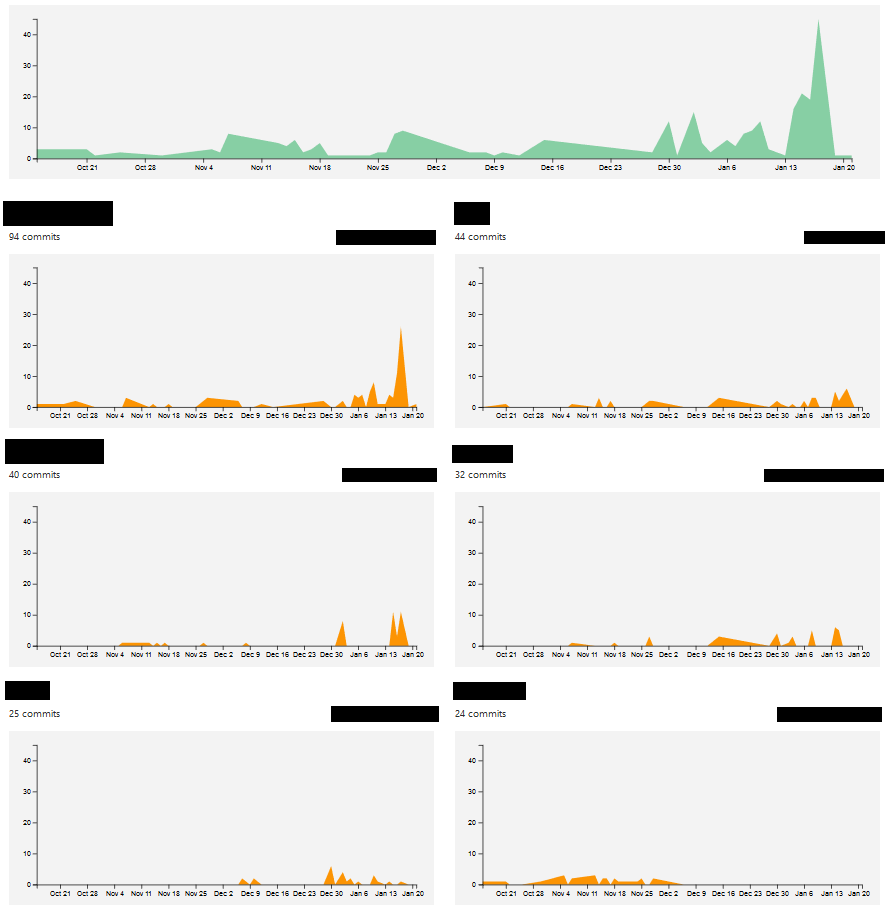
\includegraphics[scale=0.4]{slike/aktivnost.PNG} %veličina slike u odnosu na originalnu datoteku i pozicija slike
			\centering
			\caption{Primjer slike s potpisom}
			\label{fig:promjene}
		\end{figure}
		
		\begin{figure}[H]
			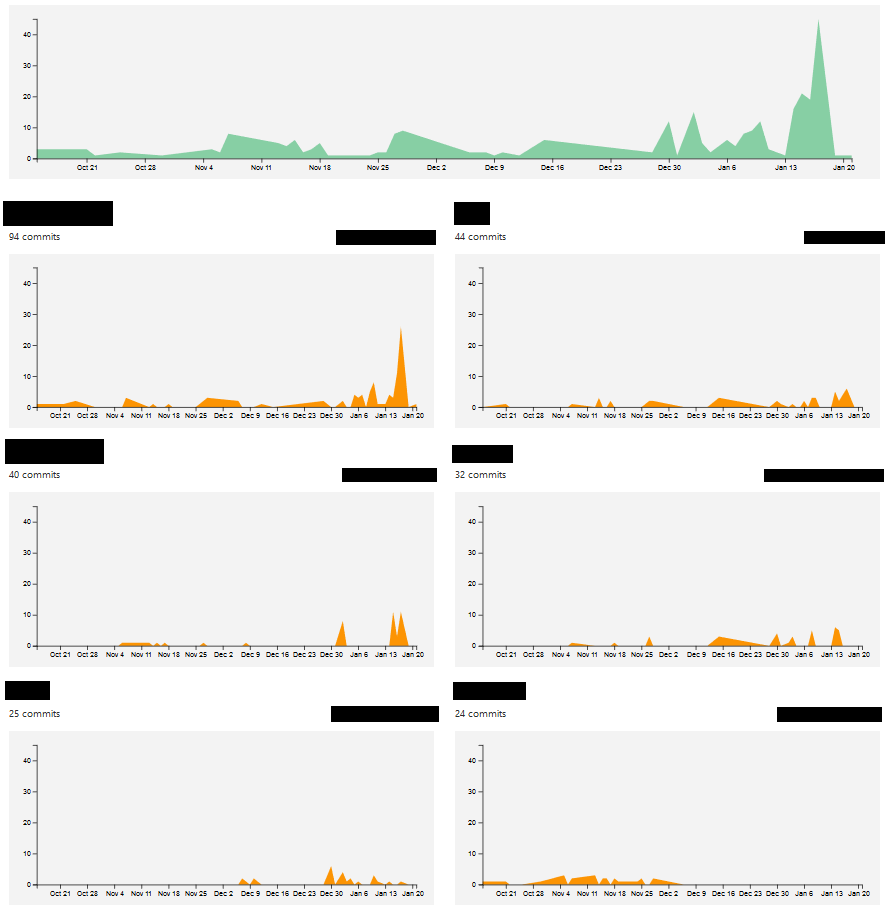
\includegraphics[width=\textwidth]{slike/aktivnost.PNG} %veličina u odnosu na širinu linije
			\caption{Primjer slike s potpisom 2}
			\label{fig:promjene2} %label mora biti drugaciji za svaku sliku
		\end{figure}
		
		Referenciranje slike \ref{fig:promjene2} u tekstu.
		
		\eject
		
	